% Copyright 2007 by Till Tantau
%
% This file may be distributed and/or modified
%
% 1. under the LaTeX Project Public License and/or
% 2. under the GNU Public License.
%
% See the file doc/licenses/LICENSE for more details.


\lecture[26]{Using linear regression}{lecture-text}

\subtitle{confidence intervals, outliers, and leverage}

\date{5 December 2013}

% pp. 505-527


\begin{document}

\begin{frame}
  \maketitle
\end{frame}


\begin{frame}\frametitle<presentation>{Outline}
  \tableofcontents
\end{frame}


\section{The linear model}

%%%%%%
\begin{frame}{Conditional means, SDs}

  \begin{block}{Notation}
    \begin{align*}
      \mu_{Y|X} &= \; \text{mean value of $Y$ given $X$} \\
      \sigma_{Y|X} &= \; \text{SD of $Y$ given $X$} \\
    \end{align*}
  \end{block}


    \vspace{2em}

    \structure{Example:}
    Drug dose ($X$) and blood pressure ($Y$) in patients. \\
    $\mu_{Y|X}$ is the mean blood pressure among patients with dose $X$; \\
    $\sigma_{Y|X}$ is the SD.

\end{frame}

%%%%%%
\begin{frame}{The linear model}

  \structure{In words,} the values of $Y$ are normally distributed with mean
  a linear function of $X$ and a standard deviation that does not depend on $X$:
  \begin{align*}
    \mu_{Y|X} &= \beta_0 + \beta_1 X \\
    \sigma_{Y|X} &= \sigma_\epsilon
  \end{align*}
  or, equivalently,
  \begin{align*}
    Y = \beta_0 + \beta_1 X + \epsilon \\
    \epsilon \; \text{independent, with SD $\sigma_\epsilon$} .
  \end{align*}

\end{frame}


%%%%%%
\begin{frame}{Why linear?}

  \begin{enumerate}
      
    \item It is arguably the simplest possible relationship between $X$ and $Y$,
      requiring only two parameters ($b_0$ and $b_1$)

    \item Most things look linear at the right level of approximation.

    \item The mathematics works out nicely.

    \item Nonlinear relationships can often be transformed to linear relationships.

  \end{enumerate}

\end{frame}


\section{Estimates from data}


%%%%%%
\begin{frame}{Conditions}

  We clearly need some sort of \structure{independence} in the $(X,Y)$ data to make good estimates.

    \vspace{2em}

    \begin{block}{Random Subsampling Model}
      Each observed pair $(x_i,y_i)$ can be regarded as having $y_i$ sampled
      at random from the \alert{conditional} population of $Y$ values having the $X$ value $x_i$,
      and independent of the other samples.
    \end{block}

    \vspace{2em}

    \structure{Examples:}
    \begin{itemize}
      \item Heights ($X$), weights ($Y$) of a random sample from a populations.
      \item Clotting rate ($Y$) after a dose ($X$) of warfarin was administered,
        with dose assigned randomly.
    \end{itemize}

\end{frame}

%%%%%%
\begin{frame}{Parameter estimates}

  If the random subsampling model holds, then
  \begin{enumerate}
    \item[$b_0$] is an estimate of $\beta_0$ (the intercept)
    \item[$b_1$] is an estimate of $\beta_1$ (the slope)
    \item[$s_e$] is an estimate of $\sigma_\epsilon$ (the SD of the noise)
  \end{enumerate}

\end{frame}

\section{Prediction}

%%%%%%
\begin{frame}{Example:}

  Son's height ($Y$) and ``midparent'' height (average of: father's and 1.08 $\times$ mother's heights)
  (Galton 1885):
  \begin{center}
    \includegraphics<1>{galton.pdf}
    \includegraphics<2>{galton-mean.pdf}
    \includegraphics<3>{galton-pred.pdf}

  \only<2>{\structure{Error} size $\approx \sigma_Y$}
  \only<3>{\structure{Error} size $\approx \sigma_\epsilon < \sigma_Y$}
  \begin{align*}
    \mu_X &= 68.09 & \sigma_X &= 2.52 \\
    \mu_Y &= 68.31 & \sigma_Y &= 1.79 \\
    r &= 0.459 & s_e &= 2.24 
  \end{align*}
  \end{center}

\end{frame}


\section{Inference on the slope}

%%%%%%
\begin{frame}{The standard error of the slope}

  Recall that $b_1$ is our \structure{estimate} for the slope $\beta_1$.

  \begin{block}{Standard Error for $b_1$}
      \[
          \SE_{b_1} = \frac{ s_e }{ s_x \sqrt{n-1} }
      \]
  \end{block}

    \vspace{2em}
    
    \only<1>{
        \begin{center}
        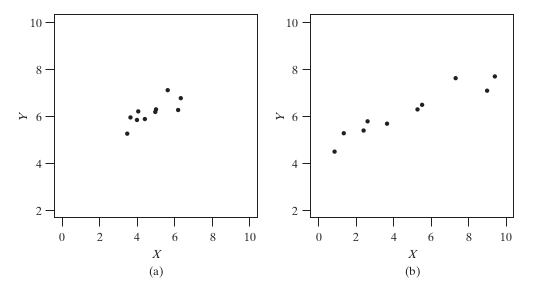
\includegraphics[width=3in]{fig-12-5-1.png}
        \end{center}
    }
    \pause

    This quantifies the intuition that
    we will be more certain about the relationship with
    \begin{itemize}
        \item less noise in the relationship ($s_e$)
        \item larger sample size ($n$)
        \item a wider spread of $x$ values ($s_x$)
    \end{itemize}

    \vspace{2em}

    A 95\% confidence interval for the slope is then
    \[
        b_1 \pm t_{n-2,0.025} \SE_{b_1} .
    \]

\end{frame}


%%%%%%
\begin{frame}{Hypothesis testing}

    We can do as usual with $\SE_{b_1}$:
    under a null hypothesis of no relationship
    \[
        H_0: \; \beta_1 = 0
    \]
    the test statistic 
    \[
        t_s = \frac{b_1 - 0}{\SE_{b_1}}
    \]
    is $t$-distributed with $n-2$ degrees of freedom.

    \vspace{2em}

    \structure{Note:} this is the \alert{same} as our previous test of no correlation.

\end{frame}


%%%% %%%%%%% %%%%%%%
\section{Interpretation}


%%%%%%
\begin{frame}{Nonlinearity}

    \begin{center}
    \includegraphics<1>{nonlinear1.pdf}
    \includegraphics<2>{nonlinear2.pdf}
    \end{center}

    If the true relationship isn't linear, then linear regression might not be the right tool.


\end{frame}

% %%%%%%
% \begin{frame}{Transformation example}
% 
% \end{frame}


%%%%%%
\begin{frame}{Outliers}

    An \alert{outlier} is a data point unusually far from the rest (in some sense; usually in the sense of having \alert{large residuals}).
    \begin{center}
        \includegraphics<1>[width=3in]{fig-12-6-3.png}
        \includegraphics<2>[width=2in]{fig-12-6-3.png}
    \end{center}
    \pause

    These usually indicate deviations from the model;\\
    and may have a large effect on the results.


    \vspace{2em}

    \structure{What to do:} investigate, use robust statistics, stay skeptical.

\end{frame}


%%%%%%
\begin{frame}{Leverage points}

    A \alert{leverage point} is one that \emph{could} have a large effect on the regression.
    (i.e.\ moving it changes the slope of the regression line a lot)
    \begin{center}
        \includegraphics<1>[width=3in]{fig-12-6-3.png}
        \includegraphics<2>[width=2in]{fig-12-6-3.png}
    \end{center}
    \pause

    \vspace{1em}

    These are \structure{far from the center of mass}.


    \vspace{1em}

    \structure{What to do:} investigate, stay skeptical.

\end{frame}



%%%%%%
\begin{frame}{Influential points}

    An \alert{influential point} is one that actually \alert{is} affecting the regression line a lot -- if it was removed, the slope would change dramatically.
    \begin{center}
        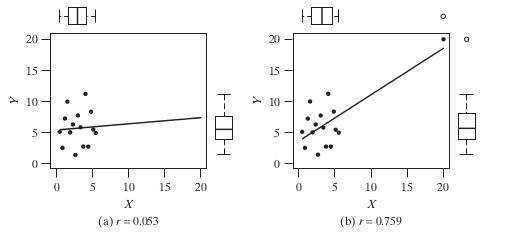
\includegraphics[width=3in]{fig-12-6-4.png}
    \end{center}

    \vspace{2em}

    \structure{What to do:} investigate, stay skeptical.

\end{frame}


%%%%%%
\begin{frame}{Nonindependence}

    Twenty measurements of serum cholesterol ($X$) and serum glucose ($Y$)
    in two humans (ten each):
    \begin{center}
        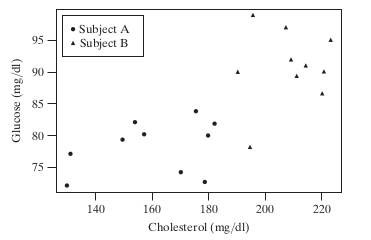
\includegraphics[width=3in]{fig-12-6-5.png}
    \end{center}

    Is the correlation significant? \\
    (How many data points are there?)

\end{frame}


\section{Diagnostic plots}


%%%%%%
\begin{frame}{Residuals versus predicted}
    Checks for nonlinearity; \uncover<3->{heteroskedasticity (different variances)}
    \begin{center}
        \includegraphics<1>{nonlinear2-resids.pdf}
        \includegraphics<2>[width=\textwidth]{usc-temps-fit-resid.pdf}
        \includegraphics<3>{hetersked-resids.pdf}
    \end{center}

    \structure{The hope} is to see \alert{no structure} in the residual plot.

\end{frame}



%%%%%%
\begin{frame}{What can go wrong?}

    \begin{center}
        \includegraphics[width=\textwidth]<1>{many-regressions-1.pdf}
        \includegraphics[width=\textwidth]<2>{many-regressions-2.pdf}
        \includegraphics[width=\textwidth]<3>{many-regressions-3.pdf}
    \end{center}

\end{frame}




\section<article>{Summary}
\section<presentation>*{Summary}

\begin{frame}{Summary}
  \begin{enumerate}
      \item Linear regression fits a model where the mean of $Y$ is a linear function of $X$
      \item and the variances do not depend on $X$.
      \item Under the ``random subsampling model'',
      \item $b_0$ and $b_1$ are good estimates of the terms in the linear relationship
      \item and $s_e$ is a good estimate of the residual SD.
      \item Testing for correlation is equivalent to testing for $b_1=0$,
      \item which we can do with a $t$ test and $\SE_{b_1}$.
      \item Look at the data to check if the conditions are met.
  \end{enumerate}
\end{frame}

% homework
\begin{frame}{Homework}
  \begin{center}

      Two 8.5"$\times$11" pages, two-sided, of handwritten notes.

    \vspace{2em}

    Bring a calculator (besides your phone).

  \end{center}
\end{frame}


\end{document}





